\section{Norms, exact quadratic degree and oscillating genus ratios}
\label{cmextend:sec:extensions}
The fixed-field formula gives sharper arithmetic information at multiples
of twelve. Together with the lattice bounds used for CM nonvanishing, it
also proves that the recorded quadratic fields are attained at every even
weight. These are further consequences developed from the incoming genus
and modular-polynomial results.

\begin{theorem}[Quadratic norm at every weight divisible by twelve]
\label{cmextend:thm:norm12}
Under the hypotheses of the genus theorem, put $K=\Q(\sqrt e)$ and let
$\sigma$ be its nontrivial automorphism. For every integer $m\ge1$,
\[
 R_{12m}(D)\in K_{>0},\qquad
 \sigma(R_{12m}(D))=\frac{A_\varepsilon^{12m}}{R_{12m}(D)}>0,
 \qquad N_{K/\Q}(R_{12m}(D))=A_\varepsilon^{12m}.
\]
Thus $A_\varepsilon^{-6m}R_{12m}(D)$ is a totally positive norm-one
element of $K$. No integrality or unit assertion is implicit.
\end{theorem}
\begin{proof}
In \eqref{cmgenus:eq:noroot}, weight $12m$ has $a=b=0$. Write
$B=A_\varepsilon^6u_e^{-t}$, where
$t=12h(e)\lambda_-=24h(e)h(D_-)/\omega(D_-)$.
This is an even integer: the unit counts $\omega(D_-)=2,4,6$ give
respectively factors $12,6,4$. Since $N(u_e)=\pm1$,
\[
 \sigma(B)=A_\varepsilon^6u_e^t,\qquad N(B)=A_\varepsilon^{12}.
\]
The two genus factors are exchanged by $\sigma$. Since $P_{12m}$ has
rational coefficients, their resultant quotient $x\in K^\times$ satisfies
$\sigma(x)=1/x$. Both real embeddings of $x$ have the same sign, so
$\sigma(|x|)=1/|x|$. This last conclusion uses the reciprocal identity;
absolute value does not generally commute with arbitrary field embeddings.
Now $R_{12m}=B^m|x|$, and multiplication proves all statements.
The CM nonvanishing theorem makes every quotient nonzero.
\end{proof}

\begin{theorem}[Exact quadratic degree at all even weights]
\label{cmextend:thm:exactdegree}
For $D=-15,-20,-39$ and every even $w\ge4$, respectively,
\[
 R_w(D)\in\Q(\sqrt5)\setminus\Q,\quad
 R_w(D)\in\Q(\sqrt5)\setminus\Q,\quad
 R_w(D)\in\Q(\sqrt{13})\setminus\Q.
\]
Each ratio is totally positive in its quadratic field, and
\[
 N(R_w(-15))=N(R_w(-20))=2^{-w},\qquad
 N(R_w(-39))=(3/4)^w.
\]
\end{theorem}
\begin{proof}
Quadratic closure follows from the preceding seed theorem. The explicit
seed ratios are totally positive and have norms $A_\varepsilon^4$ and
$A_\varepsilon^6$. Formula~\eqref{cmgenus:eq:noroot} and the reciprocal
resultant argument just used therefore give total positivity and norm
$A_\varepsilon^w$ at every even weight. If a ratio were rational, its
positivity and norm would force $R_w=A_\varepsilon^{w/2}$.

We exclude that value by uniform rational lattice bounds. At $D=-15$,
the absolute fourth-power lattice sum for $(2,1,2)$ is less than $8$;
at $D=-20$, that for $(2,2,3)$ is less than $5$. Every nonzero vector in
a reduced lattice has length at least one, so these are upper bounds for
the absolute sums at all even $w\ge4$. Combine them with the principal
lower bound $7/20$ to get
\[
 R_w(-15)>7/160>2^{-5},\qquad
 R_w(-20)>7/100>2^{-4}.
\]
They exclude rationality for $w\ge10$ and $w\ge8$, respectively.
At $D=-39$, the weight-twelve tails after removing the two axis unit
vectors are less than $1/2,1/2,3/4$ at forms $(1,1,10),(2,1,5),(3,3,4)$.
All remaining vectors have length greater than one. The same bounds hold
at every $w\ge12$, and give
\[
 R_w(-39)>\frac{(3/2)(5/4)}{(5/2)^2}=3/10
                  >(3/4)^6\ge(3/4)^{w/2}.
\]
The conjugate pair of forms with $a=2$ has equal absolute values, which
explains the squared denominator.

These five lattice caps are certified by the finite rectangle
$|n|\le10$, $|m|\le20$ and the tail estimates from the nonvanishing proof.
For a twelfth-power sum the layer-cake integral is
$63\pi/(256A^{11})$; using $\pi<4$ gives the $n$-tail
$2/(11N^{11})+63/(320N^{10})$. The $m$-tail is
$4N/[11(M-N/2)^{11}]$, with the additional axis tail
$2/(11M^{11})$. The fourth-power cap at $(2,1,2)$ uses the rational
imaginary lower bound $9/10$; all other caps use one. The exact fractions
and comparisons are retained in \texttt{verification/CM-genus-extensions.json}.

The only smaller weights left are $4,6,8$, and where needed $10$.
The seed formulas at $4,6$ have nonzero radical coefficients, and
$R_8=R_4^2$, $R_{10}=R_4R_6$ have positive radical coefficients as well.
Thus none is rational. This proves exact degree two at every stated weight.
\end{proof}

\subsection{New explicit quadratic evaluations}
The reduced polynomials give nine further formulas at weights $12,16,18$.
For instance,
\begin{align}
 R_{12}(-15)&=\frac{34829+15576\sqrt5}{1216},
       \label{cmextend:eq:r12d15}\\
 R_{16}(-15)&=\frac{307761+137632\sqrt5}{511744},\\
 R_{18}(-15)&=\frac{64494289+28842228\sqrt5}{193434112}.
\end{align}
For the other two discriminants the complete coefficients are recorded as
rational pairs in \texttt{verification/CM-genus-extensions.json}. These
are exact evaluations by the resultant recipe, rather than decimal fits.
In particular the first has norm $1/4096$ even though its positive
embedding is approximately $57.28$; the other embedding is very small.

\subsection{A quadratic sequence with a full interval of limit points}
The large first value is part of a structural phenomenon. Let
$\tau=(-1+i\sqrt{15})/4=e^{i\theta}$, and write $r_m=R_{12m}(-15)$.

\begin{theorem}[The cluster set at discriminant $-15$]
\label{cmextend:thm:cluster}
The finite limit points of $r_m$, as $m\to\infty$, are precisely
$[1/2,\infty)$. Also
\[
 \liminf_{m\to\infty}r_m=1/2,\qquad
 \limsup_{m\to\infty}r_m=\infty,\qquad
 \sigma(r_m)=2^{-12m}/r_m\longrightarrow0.
\]
Thus exact quadratic degree at every weight coexists with dense limiting
behavior in one embedding and exponential decay in the other.
\end{theorem}
\begin{proof}
The principal lattice has only the unit vectors $\pm1$, and all other
vectors have length greater than one. Its row sum tends to two.
In the second lattice the unit vectors are exactly $\pm1,\pm\tau$;
the next length is $\sqrt{3/2}$. Absolute convergence at weight four
therefore gives the additive estimate
\[
 G_{12m}(\tau)=2+2\tau^{-12m}+O((3/2)^{-6m}),
 \qquad |G_{12m}(\tau)|=4|\cos(6m\theta)|+O((3/2)^{-6m}).
\]
The error is additive; it is not divided by a small cosine.

The angle $\theta/\pi$ is irrational. Otherwise $\tau$ would be a root
of unity, making $\tau+\tau^{-1}=-1/2$ an algebraic integer, which is
impossible for that rational number. Thus $6m\theta$ is dense modulo
$\pi$. Along a subsequence with $|\cos(6m\theta)|\to c>0$,
$r_m\to1/(2c)$, giving every finite limit in $[1/2,\infty)$.
Along a subsequence with the cosine tending to zero, the denominator
tends to zero while the numerator tends to two; CM nonvanishing makes
each term defined, so $r_m\to\infty$. The upper bound
$|G_{12m}(\tau)|\le4+o(1)$ excludes finite limit points below $1/2$.
Finally the norm theorem gives the conjugate formula, and the positive
lower bound on $r_m$ proves its convergence to zero.
\end{proof}

\begin{figure}[htbp]
\centering
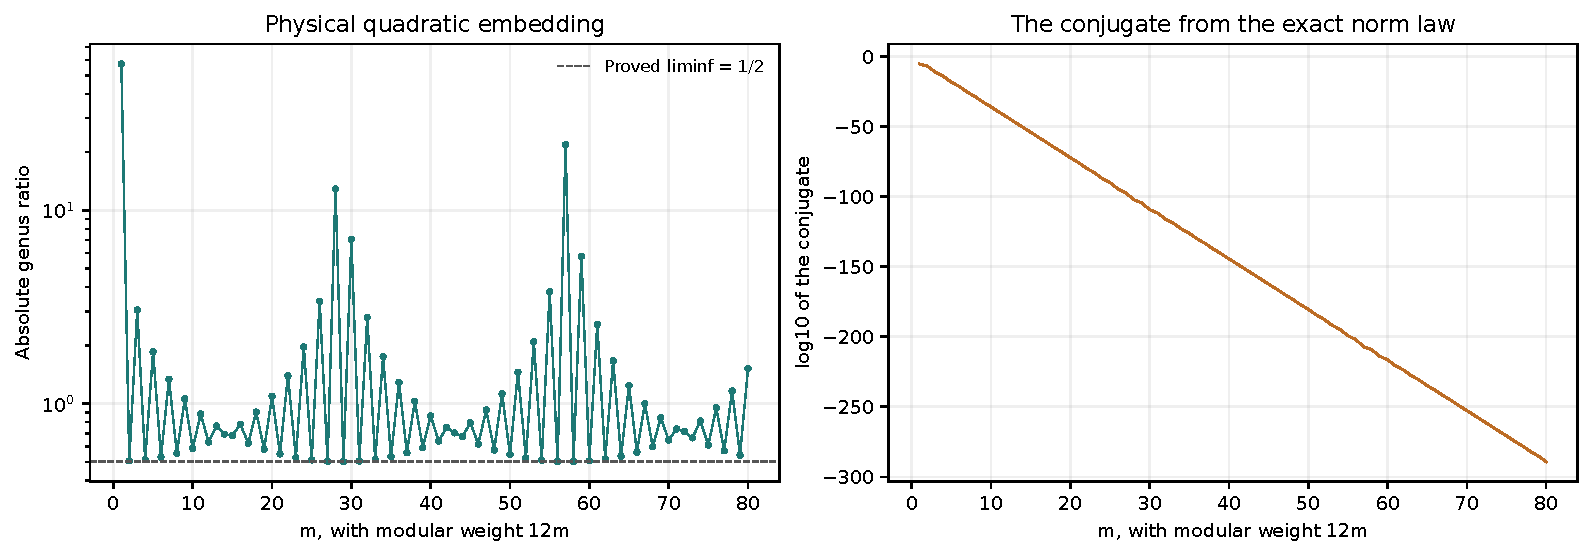
\includegraphics[width=\textwidth]{figures/cm_genus_embeddings.pdf}
\caption{Numerical illustrations of the proved genus-ratio behavior at
$D=-15$. The physical embedding has large oscillations; its quadratic
conjugate is computed from the exact norm law. Finite lattice sums supply
the plotted values and explicit analytic tail budgets. The cluster theorem,
not these finitely many points, proves the full interval of limit points.}
\label{cmextend:fig:embeddings}
\end{figure}
